\documentclass[a4paper, a4wide]{article}
\usepackage{url}
\usepackage{listings}
\usepackage{graphicx}

\begin{document}

\lstset{language=bash}
\lstset{basicstyle=\ttfamily, columns=fixed, breaklines=true}

\title{A brief guide for AFiVO}
\author{Jannis Teunissen}
\maketitle

\section{Introduction}
\label{sec:introduction}

Afivo (Adaptive Finite Volume Octree) is a framework that provides the basics
for finite volume simulations with adaptive mesh refinement.
There are already a number of such frameworks available, but Afivo is different
in a couple of ways.
For one, it provides less functionality.
This means that there is less code, which should makes it easier to modify
things yourself.

Here are some of other the features of Afivo:

\begin{itemize}
  \item Afivo is designed for OpenMP parallelism (shared memory systems).
  \item Afivo comes with a FAS multigrid solver.
  \item Afivo can write VTK output which can be visualized with many tools,
  e.g., Visit.
  \item Afivo supports 2D and 3D meshes.
  \item Afivo is written in \emph{modern} Fortran, and uses some Fortran 2008
  features.
  However, we do not use an object-oriented approach.
\end{itemize}

This document can help you get started with Afivo. However, to really learn how
to use it, you should probably look at some of the code yourself, maybe starting
out with the examples. It can also be helpful to use the doxygen documentation,
which can be generated by typing \texttt{doxygen} in the Afivo folder (of course,
you need to have doxygen installed). Then, you can open the html documentation
in any browser (\texttt{doc/html/index.html}).

Also note that this short guide addresses most things in 2D, because that is
often a bit simpler, but everything should work in the same way if you change
2(D) to 3(D).

\section{Quadtree / octree meshes}
\label{sec:amrmesh}

Afivo uses 2:1 balanced quadtree (2D) / octree (3D) meshes, in much the same way
as Paramesh does.
Such meshes can be described by the following rules:

\begin{itemize}
  \item The mesh is constructed from boxes that contain $N^d$ cells, where $d$
  is the number of coordinates.
  \item Boxes can be refined by a factor of two, in which case $2^d$ refined
  boxes are created.
  \item The difference in refinement level for adjacent boxes is at most one.
\end{itemize}

In figure \ref{fig:example-quadtree} you can see some examples of a quadtree
mesh that gets refined.
The \emph{tree} in quadtree / octree refers to the fact that such meshes are
often represented as trees, in which the children of a node (which represents a
box) are the refinements of the box.

\begin{figure}
  \centering
  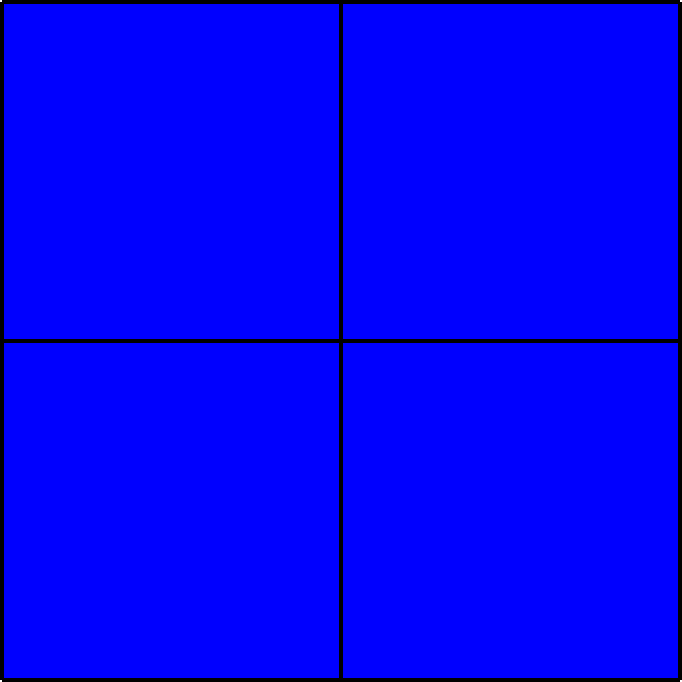
\includegraphics[width=2.5cm]{figures/quadtree_cex1.png}
  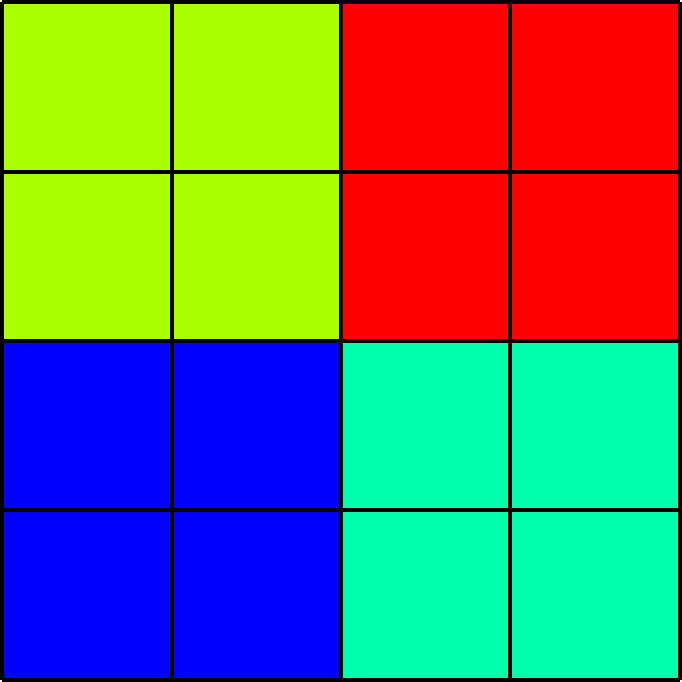
\includegraphics[width=2.5cm]{figures/quadtree_cex2.png}
  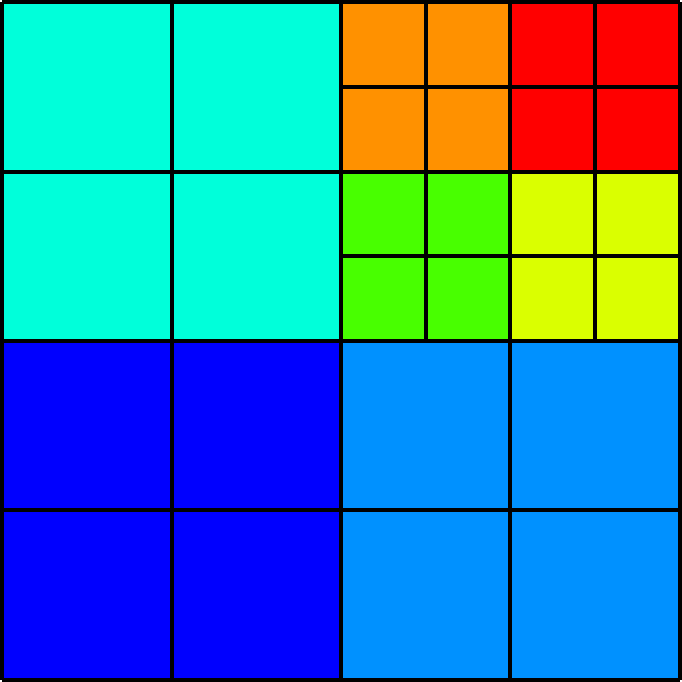
\includegraphics[width=2.5cm]{figures/quadtree_cex3.png}
  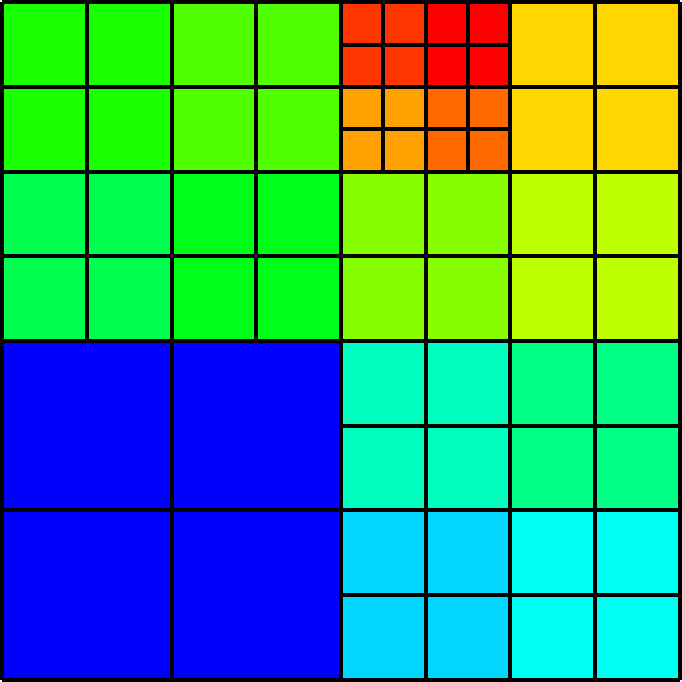
\includegraphics[width=2.5cm]{figures/quadtree_cex4.png}
  \caption{Examples of a quadtree mesh that gets refined.
    Here boxes contain $2 \times 2$ cells, and different boxes have different
    colours. Note that in the rightmost picture, there are so many boxes that
    differences in colour are hardly visible.}
  \label{fig:example-quadtree}
\end{figure}

\section{Getting and compiling Afivo}
\label{sec:getting-started}

\subsection{Obtaining the code}
\label{sec:obtaining}

Afivo can be obtained from \url{https://github.com/jannisteunissen/afivo}. If
you have git installed, simply clone the repository like this:

\begin{lstlisting}
  git clone https://github.com/jannisteunissen/afivo
\end{lstlisting}

\subsection{Compiling the code}
\label{sec:compilation}

Compilation requires a relatively new gfortran compiler\footnote{ifort is also
  supported, use \texttt{make COMPILER=ifort}}, and should then be as simple as
this:
\begin{lstlisting}
  cd afivo
  make
\end{lstlisting}
This will create a file \texttt{libAfivo.a} in the \texttt{src} directory, which
you can link to from your own code.
For that you typically need the module\footnote{The Fortran equivalent of header
  files} files, which are also in the \texttt{src} directory.
Furthermore, the examples that come with Afivo will be compiled, and the
executables can be found in the \texttt{examples} directory.

\lstset{language=[08]Fortran}
\section{An example of an Afivo mesh}
\label{sec:examples}

In the \texttt{examples} directory you can find the
examples that come with Afivo.
Here we discuss some of them.
The examples produce output in the VTK unstructured format (XML
type\footnote{See \url{http://www.vtk.org/VTK/img/file-formats.pdf} for a
  specification}).
You can visualize these files with for example Visit\footnote{Visit can be
  obtained from \url{https://wci.llnl.gov/simulation/computer-codes/visit}}.

\subsection{Constructing a simple mesh}
\label{sec:example-base}

The first example that we discuss is \texttt{test\_base\_2d.f90}.
There is also a 3D version (\texttt{test\_base\_3d.f90}).

Let us go through the important bits of code.
First, we create a variable \texttt{tree}, which will later contain the complete
mesh with all its data.
Then we need to tell Afivo some of the properties of the mesh, to initialize the
\texttt{tree}.

\begin{lstlisting}
  type(a2_t) :: tree

  ! Initialize tree
  call a2_init(tree, & ! Tree to initialize
       box_size, &     ! Number of cells
       n_var_cell, &   ! Number of face-centered vars
       n_var_face, &   ! Number of cell-centered vars
       dr)             ! Distance between coarse cells
\end{lstlisting}

For example, in figure \ref{fig:example-quadtree}, \texttt{box\_size} was set to
two. Here we set it to eight.
Now that we have defined the basic properties of a box, let's add two boxes to
the mesh.
We have to define where a box is (a spatial index), and what its neighbors
are.
This is done in the following way
\begin{lstlisting}
  ix_list(:, 1) = [1,1] ! One box at 1,1
  ix_list(:, 2) = [2,1] ! One box at 2,1

  ! Set neighbors for box one
  nb_list(a2_nb_lx, 1) = 2
  nb_list(a2_nb_hx, 1) = 2
  nb_list(a2_nb_ly, 1) = 1
  nb_list(a2_nb_hy, 1) = 1

  ! Set neighbors for box two
  nb_list(:, 2) = 2

  ! Create the base mesh
  call a2_set_base(tree, ix_list, nb_list)
\end{lstlisting}

\begin{figure}
  \centering
  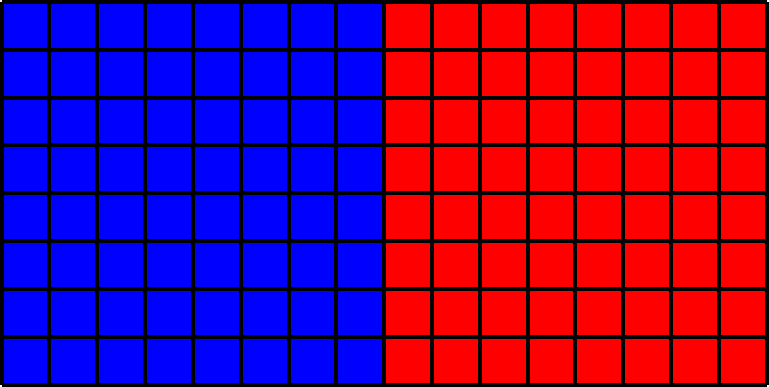
\includegraphics[width=7.5cm]{figures/two_boxes.png}
  \caption{Two boxes of $8 \times 8$ cells, with periodic boundary conditions on
  the outside.}
  \label{fig:two-boxes}
\end{figure}

The result is shown in figure \ref{fig:two-boxes}.
In two dimensions, a spatial index consists of two indices.
See figure \ref{fig:box-indices} for an example.
In Afivo, boxes should have positive spatial indices, so (1,1) is the lowest
index you can give.

\begin{figure}
  \centering
  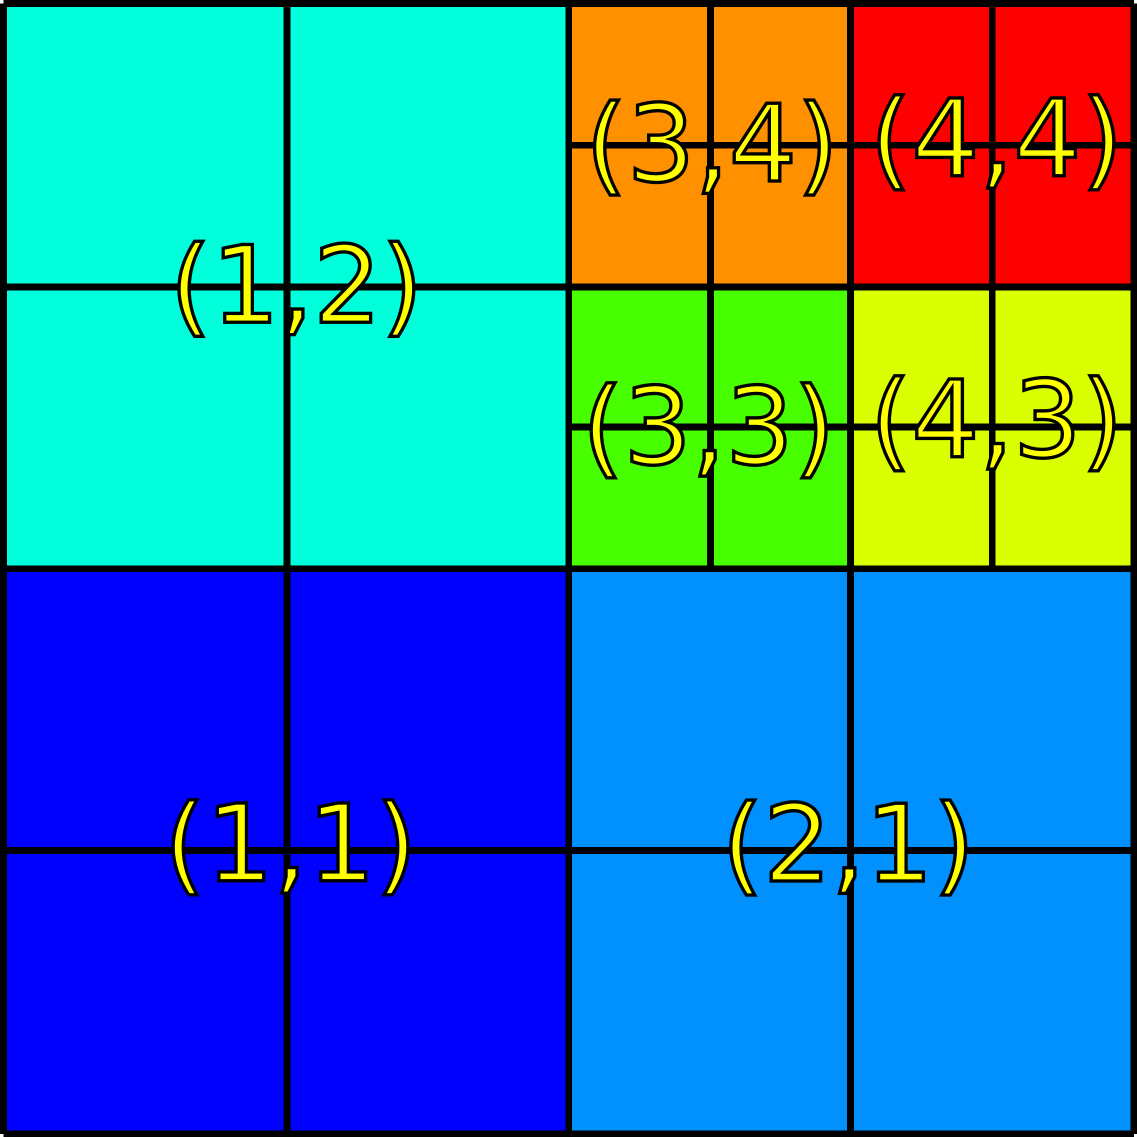
\includegraphics[width=7.5cm]{figures/box_indices.png}
  \caption{An example which shows the spatial indices of boxes that contain
    $2 \times 2$ cells.
    Below the four boxes in the top-right corner lies a (2,2) coarse box.}
  \label{fig:box-indices}
\end{figure}

In two dimensions, a box has four neighbors, which are ordered as lower-x,
higher-x, lower-y, higher-y (and lower-z, higher-z in 3D).
Here we create two boxes next to each other, with periodic boundary conditions.
Note that we do not need to specify all the neighbors for box two, because Afivo
is smart enough to understand that if box one has box two has a neighbor, then
that should also be true vice-versa.

\subsection{Refining the mesh}
\label{sec:refining-mesh}

The mesh that we've constructed thus far is shown in figure \ref{fig:two-boxes}.
In order to refine it, we do the following:
\begin{lstlisting}
  call a2_adjust_refinement(tree, set_ref_flags, ref_info)
\end{lstlisting}
After the call, \texttt{ref\_info} contains the total number of new and removed
boxes, as well as the indices of the new and removed boxes per refinement level.

The user's refinement routine is called for each box.
The routine gets a list of all boxes, the id of the current box, and a list with
all the refinement flags.
In this way, you can for example specify that the current box and its left
neighbor should be refined\footnote{In parallel different flags might be
  specified for the same box.
  In that case, Afivo picks the \emph{highest} flag (refine $>$ keep refinement
  $>$ derefine).
  If you don't set refinement flags for a box, it will keep its refinement.}, or
you can use data at a neighbor when deciding whether or not to refine the
current box.

A refinement flag can have three values:
\begin{itemize}
  \item \texttt{a5\_kp\_ref} keep refinement as is
  \item \texttt{a5\_do\_ref} refine
  \item \texttt{a5\_rm\_ref} derefine
\end{itemize}
The refinement function in our example is particularly simple, because it
refines or derefines based on a random number:
\begin{lstlisting}
  subroutine set_ref_flags(boxes, id, ref_flags)
    type(box2_t), intent(in) :: boxes(:)
    integer, intent(in)      :: id
    integer, intent(inout)   :: ref_flags(:)
    real(dp)                 :: rr

    call random_number(rr)
    if (rr < 0.2_dp .and. boxes(id)%lvl < 10) then
       ref_flags(id) = a5_do_ref
    else
       ref_flags(id) = a5_rm_ref
    end if
  end subroutine set_ref_flags
\end{lstlisting}

It is important to understand two things about \texttt{a2\_adjust\_refinement}:
First, it will change the refinement level at some location by at most one.
So sometimes, you will need to call it multiple times.
Second, it will sometimes refine areas that you did not specify for refinement,
to ensure 2:1 balance (no jumps in refinement level).
So the good news is that when you write your refinement function, you do not
need to worry about this.

In figure \ref{fig:random-refinement}, the result is shown after 8 steps of
random refinement.
Note that 2:1 balance is also preserved along the periodic coordinates.

\begin{figure}
  \centering
  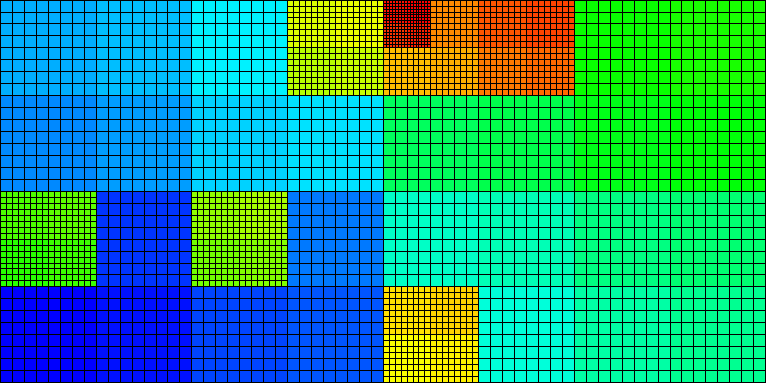
\includegraphics[width=7.5cm]{figures/random_ref.png}
  \caption{Random refinement}
  \label{fig:random-refinement}
\end{figure}

\section{Data structures: boxes, levels and trees}
\label{sec:data-structures}

Of course, we do not only want to define a mesh, but we also want to do
computations on it. Therefore, let us have a look at the different data
structures used in Afivo.

\subsection{Box type}
\label{sec:box-type}

First there is the box type, which contains the following information:
\begin{itemize}
  \item lvl: the refinement level of the box
  \item tag: Afivo (and you) can set bits in this integer to store information
  about the box.
  \item ix: the spatial index of the box
  \item parent: the parent of the box
  \item children: the children of the box
  \item n\_cell: the number of cells along each coordinate of the box
  \item r\_min: the minimum coordinate of the box
  \item cc: array of dimension $d+1$ that can store multiple cell-centered
  variables
  \item fx, fy, (fz): arrays of dimension $d+1$ that can store multiple
  face-centered variables or fluxes.
\end{itemize}

The parent and children of a box are referred to by positive integers.
These integers are actually just indices in an array with all the boxes, which
is stored in the tree type.

\subsection{Tree type}
\label{sec:tree-type}

The tree type contains the following data:
\begin{itemize}
  \item lvls\_max: the maximum allowed refinement level
  \item max\_lvl: the current maximum refinement level
  \item n\_cell: the number of cells along each coordinate of a box
  \item n\_var\_cell: the number of cell-centered variables
  \item n\_var\_face: the number of face-centered variables
  \item r\_base: the minimum coordinate of a box at index (1,1)
  \item n\_cell: the number of cells along each coordinate of the box
  \item lvls: an array of level types (see below)
  \item boxes: an array containing all the boxes in the mesh
\end{itemize}

\subsection{Level type}
\label{sec:level-type}

Finally, the level type contains just three things:
\begin{itemize}
  \item ids: a list of all the indices of boxes at this refinement level
  \item leaves: those ids for which the boxes do not have children (i.e., are
  not refined)
  \item parents: the ids for which the boxes do have children (i.e., are refined)
\end{itemize}

\subsection{Example: setting a variable to zero}
\label{sec:data-types-example}

So how does this work in practice? Suppose that we want to loop over all the
levels, and set the cell-centered with index 1 to zero, then we could do that in
the following way:
\begin{lstlisting}
  do lvl = 1, tree%max_lvl
    do i = 1, size(tree%lvls(lvl)%ids)
      id = tree%lvls(lvl)%ids(i)
      tree%boxes(id)%cc(:, :, 1) = 0
    end do
  end do
\end{lstlisting}
If we only wanted to loop over the \emph{leaves}, we would simply replace \texttt{ids}
by \texttt{leaves}.

For most computations, it is convenient to make use of ghost cells.
This is discussed in the next section.

\section{Ghost cells}
\label{sec:ghost-cells}

In Afivo, we have two types of variables: cell-centered variables and
face-centered variables.
For the cell-centered variables, we always use one ghost cell. The flux-centered
variables are defined between all cell-centered variables in a direction, see
figure \ref{fig:location-cc-fx}.

\begin{figure}
  \centering
  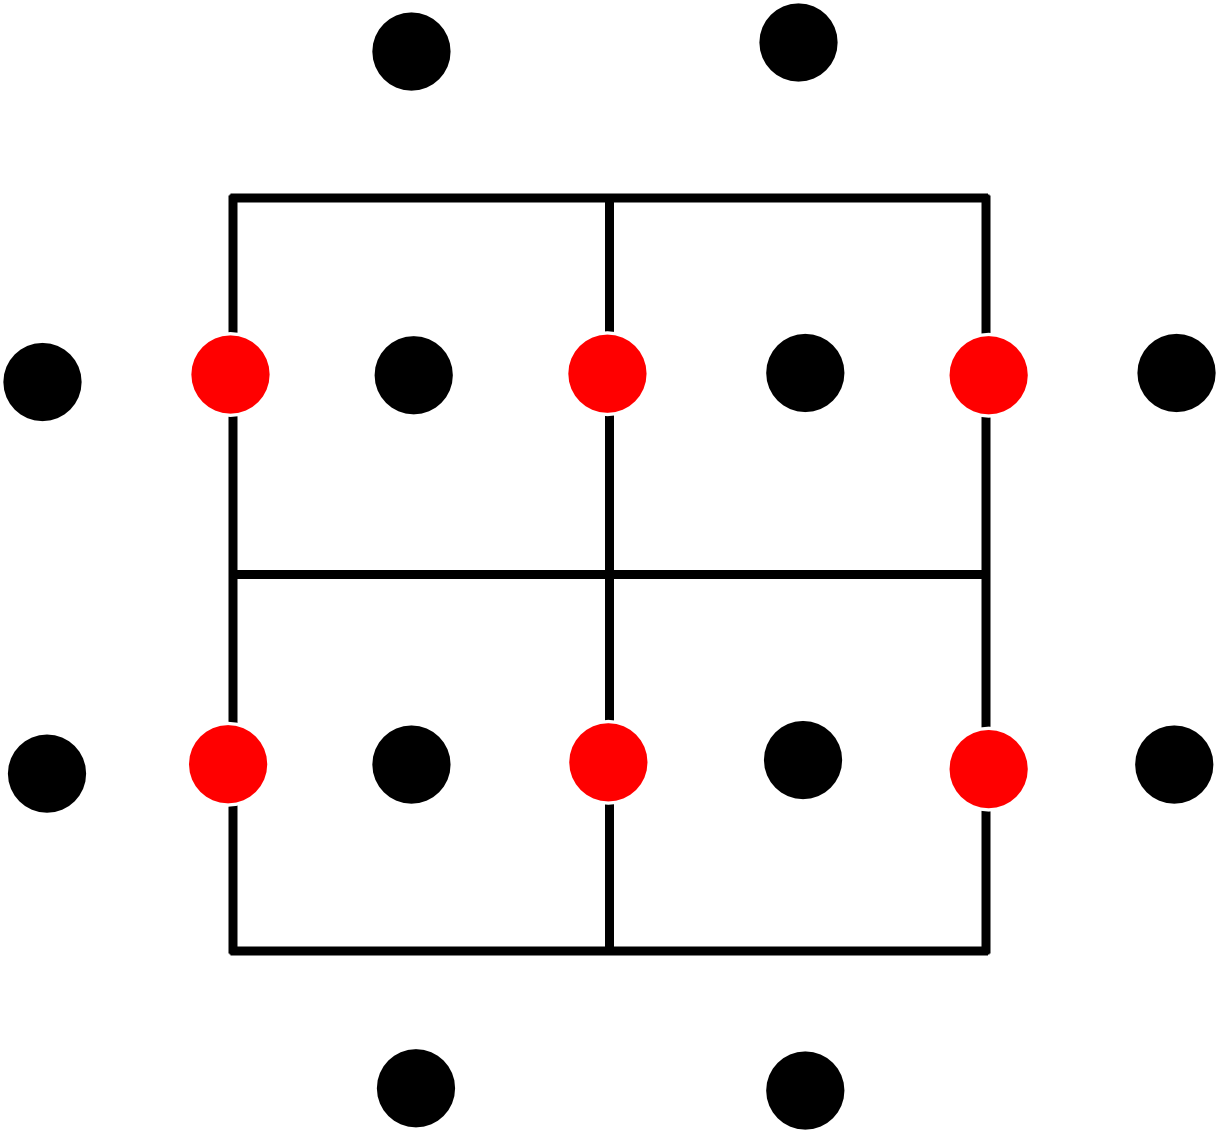
\includegraphics[width=5cm]{figures/location_cc_fx.png}
  \caption{Location of the cell-centered variables (black dots) and the
    face-centered variables in the x-direction (red dots) for a box of $2\times
    2$ cells.}
  \label{fig:location-cc-fx}
\end{figure}

Suppose that we want to set all ghost cells to zero, then we could do that for
example like this:
\begin{lstlisting}
  nc = tree%n_cell
  do lvl = 1, tree%max_lvl
    do i = 1, size(tree%lvls(lvl)%ids)
      id = tree%lvls(lvl)%ids(i)
      tree%boxes(id)%cc(0, :, 1) = 0
      tree%boxes(id)%cc(:, 0, 1) = 0
      tree%boxes(id)%cc(nc+1, :, 1) = 0
      tree%boxes(id)%cc(:, nc+1, 1) = 0
    end do
  end do
\end{lstlisting}
In a real application, ghost cells should typically be set by the following routine:
\begin{lstlisting}
  a2_gc_sides(tree, iv, subr_rb, subr_bc)
\end{lstlisting}
The first two arguments are the tree to fill ghost cells on and the index of the
cell-centered variable for which we want to set ghost cells.
The next two arguments are themselves subroutines: \texttt{subr\_rb} and
\texttt{subr\_bc}.
These subroutines will be called for filling ghost cells near refinement
boundaries and physical boundaries, respectively.
All internal ghost cells are automatically handled by Afivo.

The subroutines \texttt{subr\_rb} is called for each side of a box where there
is a refinement boundary.
Similarly, \texttt{subr\_bc} is called for each physical boundary.
These routines get the following arguments: a list with all the boxes, the id of
the box to fill ghost cells for, the direction in which we want to fill ghost
cells (e.g., lower-x, higher-x, etc.)
and the index of the variable for which we set ghost cells.

For \texttt{subr\_rb}, Afivo provides a routine that does linear interpolation,
which is called \texttt{a2\_sides\_interp} in 2D.
You are of course free to create some other routine that fits your needs better.

\subsection{An example for subr\_bc}
\label{sec:ghost-cells-example}

Here is an example of a routine that sets physical boundaries.
\begin{lstlisting}
  subroutine sides_bc_pot(boxes, id, nb, iv)
    type(box2_t), intent(inout) :: boxes(:)
    integer, intent(in)         :: id, nb, iv
    integer                     :: nc

    nc = boxes(id)%n_cell

    select case (nb)
    case (a2_nb_lx)
       ! Neumann zero
       boxes(id)%cc(0, 1:nc, iv) = &
         boxes(id)%cc(1, 1:nc, iv)
    case (a2_nb_hx)
       ! Neumann zero
       boxes(id)%cc(nc+1, 1:nc, iv) = &
         boxes(id)%cc(nc, 1:nc, iv)
    case (a2_nb_ly)
       ! Dirichlet zero at cell face
       boxes(id)%cc(1:nc, 0, iv) = &
         -boxes(id)%cc(1:nc, 1, iv)
    case (a2_nb_hy)
       ! Dirichlet 1 at cell face
       boxes(id)%cc(1:nc, nc+1, iv) = &
         2 - boxes(id)%cc(1:nc, nc, iv)
    end select
  end subroutine sides_bc_pot
\end{lstlisting}

Note that in the Dirichlet case, we have to do a small computation to get the
right boundary at the cell face, which lies in between the ghost cell and an
internal point.

\section{And now...}

This guide is still quite short, so I'll repeat the advice given at the
beginning: play with the examples, have a look at the code, and try things out!

\end{document}